\section{Results \& Discussion - Temporal Discretization}
Eulers method of discretization is considered first, figure \ref{fig:Euler1} shows Eulers schemes approximation to the function $f(x)=e^x-1$ for 4 different time steps; in the range $0\leqslant x \leqslant 5$

\begin{figure}[H]
\centering
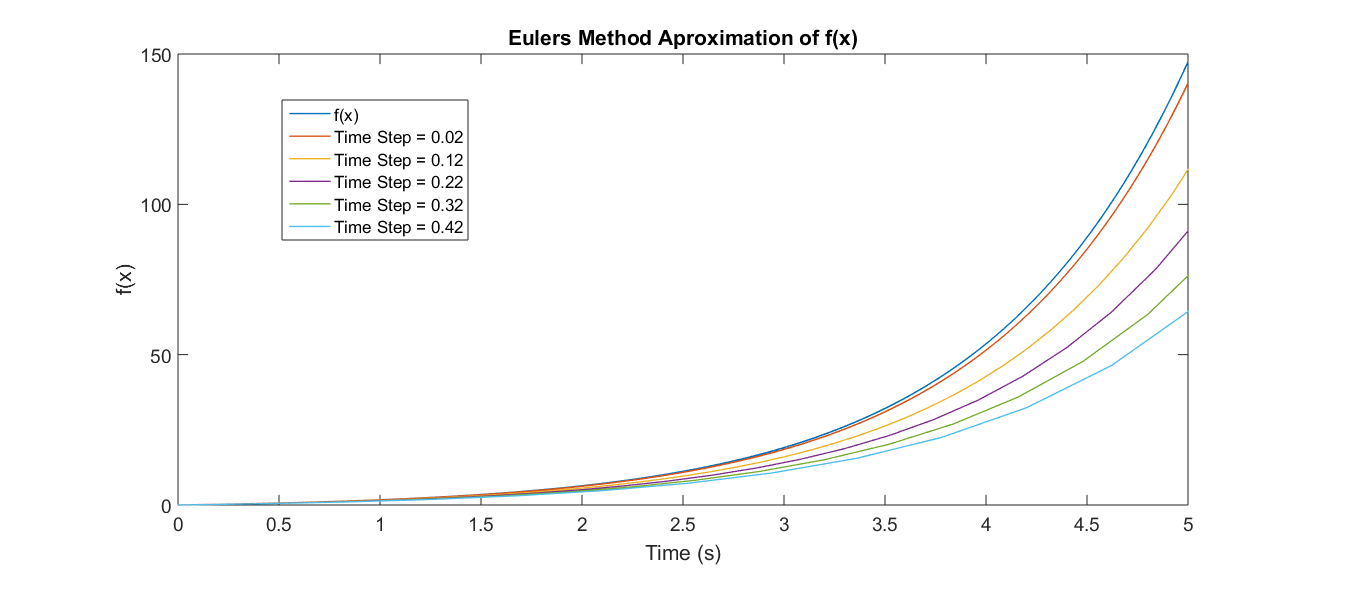
\includegraphics[width=1.0\textwidth]{Figures/EulersMethodMatlab.png}
\caption{\label{fig:Euler1} Eulers method used to approximate $f(x)=e^x-1$ for 5 different time steps}
\end{figure} 

From figure \ref{fig:Euler1} it is apparent that refining the time step increases the accuracy of the solution from the scheme. Hence Eulers method shows convergence upon $f(x)$ and would provide an accurate solution for the simulation for the current time step ($t_{ts}=0.02s$). The percent error from each time step are shown in table \ref{tab:EulerError}

\begin{table}[H]
\centering

\label{tab:EulerError}
\begin{tabular}{llllll}
\multicolumn{1}{l|}{Time Step (s)}    & 0.42 & 0.32 & 0.22 & 0.12 & 0.02 \\ \hline
\multicolumn{1}{l|}{Percent Error \%} & 54.4 & 42.4 & 34.3 & 20.8 & 4.8 
\end{tabular}
\caption{Error at $x=5$ for Eulers Method at 5 Time Steps}
\end{table}

At the default time step used by Unity, $t_{ts}=0.02s$ the error returned by Eulers method is around 5\% for a 5 second range. The time an element is likely to exist for in the simulation is likely in the same magnitude as this but considerably larger, hence the positional accuracy approximated by Eulers scheme will be larger than 5\%. This error would further propagate through the simulation as it affects the velocities calculated for all other elements.An error of around \%5 may be tolerated for the simulation to be able to run in real time however it is far from ideal. 

The next scheme to be considered is the quadratic position scheme, figure \ref{fig:Deriv1} shows the approximations to $f(x)=e^x-1$ for the same time steps and range as Eulers method was examined.

\begin{figure}[H]
\centering
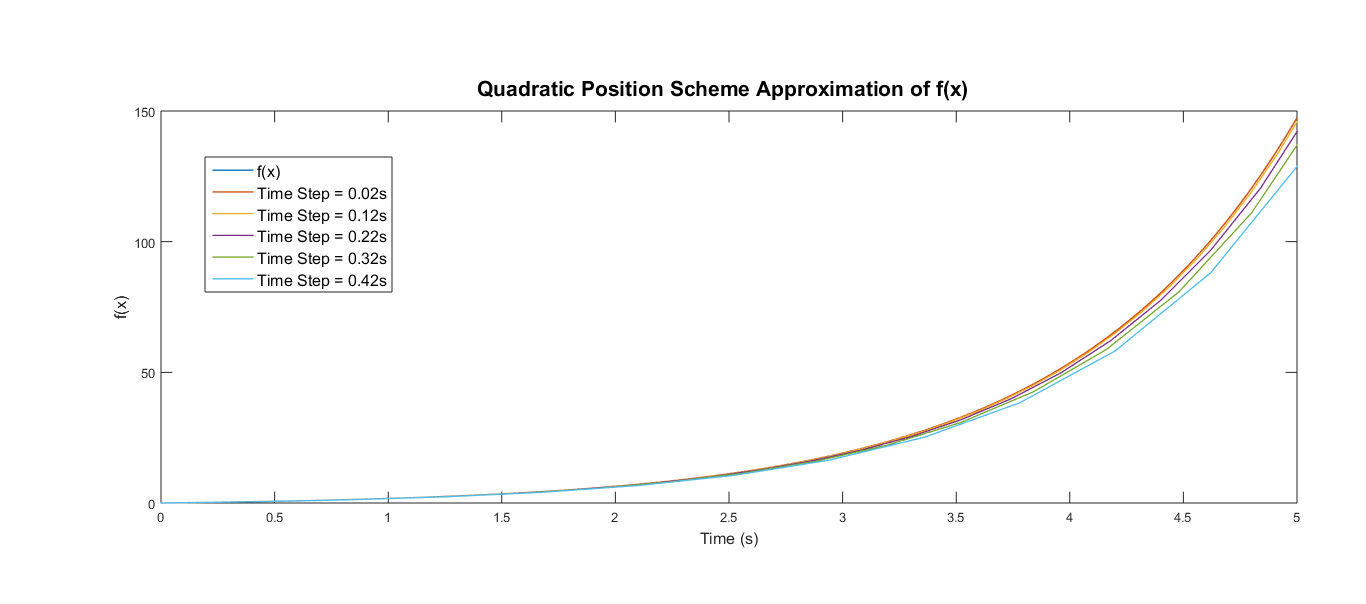
\includegraphics[width=1.0\textwidth]{Figures/DerivativeSchemeMatlab.png}
\caption{\label{fig:Deriv1} Quadratic position scheme used to approximate $f(x)=e^x-1$ for 5 different time steps}
\end{figure} 

From figure \ref{fig:Deriv1} it is apparent that the quadratic position scheme converges upon f(x), further, in contrast to figure \ref{fig:Euler1} the convergence is seen to happen at a quicker rate than Eulers method. The convergence is exhibited can be seen by the closely spaced lines of the approximation. The lines representing the approximations are so close distinguishing between them becomes difficult. The errors for the solution of $f(x)$ at $x=5$ is shown in table \ref{tab:DerivError}

\begin{table}[H]
\centering
\label{tab:DerivError}
\begin{tabular}{llllll}
\multicolumn{1}{l|}{Time Step (s)}    & 0.42 & 0.32 & 0.22 & 0.12 & 0.02 \\ \hline
\multicolumn{1}{l|}{Percent Error \%} & 9.8  & 3.4  & 1.9  & 2.8  & 0.04 
\end{tabular}
\caption{Error at $x=5$ for the Quadratic Position scheme at 5 Time Steps}
\end{table}

From these error values it is evident that the Quadratic Position scheme converges quicker than Eulers method, at $t=5$ the error is 0.04\% compared to \%4.8 for Eulers method. Note the scheme appears to diverge between time steps of $t_{ts}=0.22$ and $t_{ts}=0.12$ as the error increases, however the error then decreases from $t_{ts}=0.12$ to $t_{ts}=0.02$
\\\\
To obtain a similiar positional error as Eulers method at a time step of $t_{ts}=0.002s$ the Qudratic Positional scheme could be used with a time step of $t_{ts}=0.34$. The Quadratic Velocity scheme therefore is a more ideal scheme to use for the simulation, provided the added computational overhead from the complexity of the scheme does not outweigh the advantage of the quicker convergence.
\\\\
\begin{figure}[H]
\centering
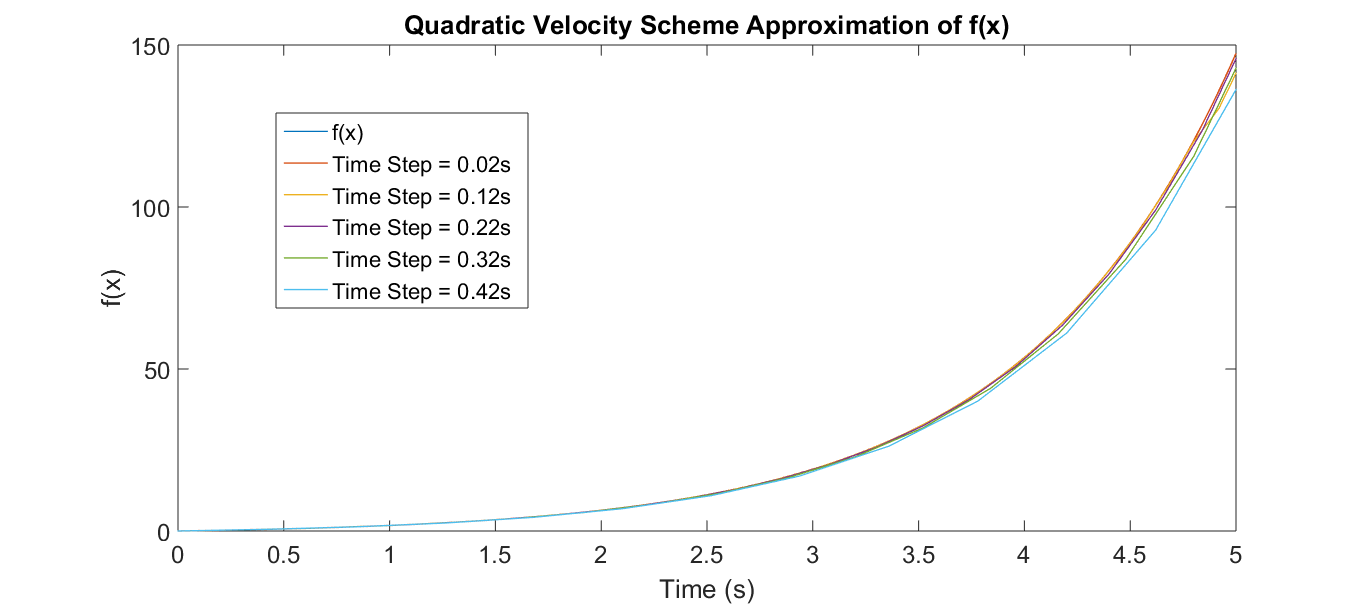
\includegraphics[width=1.0\textwidth]{Figures/QuadraticvelocityScheme.png}
\caption{\label{fig:QV1} Quadratic Velocity scheme used to approximate $f(x)=e^x-1$ for 5 different time steps}
\end{figure} 
Figure \ref{fig:QV1} shows the Quadratic Velocity schemes approximation to the function, again in for the same range and time steps. The lines representing different times steps are almost indistinguishable from each other, indicating yet a quicker rate of convergence than the Quadratic Position scheme. To quantitatively asses this the errors at $t=5$ are tabulated in table \ref{tab:QVerror}. For the smallest time step, $t_{ts}=0.02s$ the Quadratic Velocity scheme has an almost negligible error of around 0.02\%. This is far lower than both the Quadratic Position Scheme and EUler's Method. Throughout the rest of the range of time steps the Quadratic Velocity scheme results in error values similar to the Quadratic Position scheme.

\begin{table}[H]
\centering
\begin{tabular}{llllll}
\multicolumn{1}{l|}{Time Step (s)}    & 0.42 & 0.32 & 0.22 & 0.12 & 0.02  \\ \hline
\multicolumn{1}{l|}{Percent Error \%} & 7.6  & 3.1  & 1.1  & 4.2  & 0.002    
\end{tabular}
\caption{Error at $x=5$ for the Quadratic Velocity scheme at 5 Time Steps}
\label{tab:QVerror}
\end{table}

Figure \ref{fig:SchemeTime} shows a comparison of the computational time of the scheme for a range of iterations. The schemes were tested up to 25 million iterations, this was found to refer to a computational time of Eulers method of around 10 seconds. The data shows a very high degree of agreement for all 3 schemes with linear trends being apparent. Noise or other errors are apparent in some data points as they clearly deviate from the trend. However, even with this apparent the data is highly consistent with $R^2$ values of at least $R^2=0.99$ for all three data series.

\begin{figure}[H]
\centering
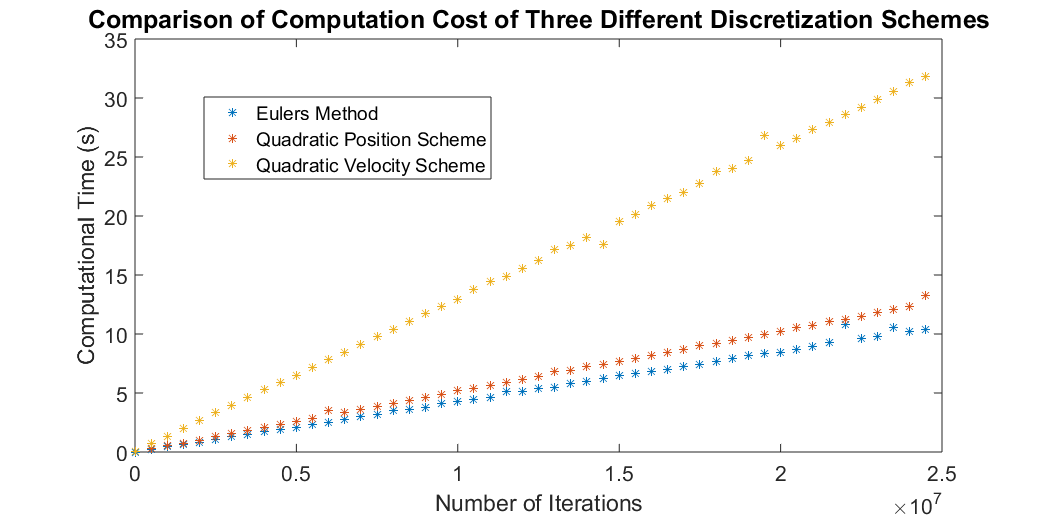
\includegraphics[width=1.0\textwidth]{Figures/SchemeComputationTime.png}
\caption{\label{fig:SchemeTime} Comparison of the Computational cost of Euler's Method, Quadratic Position scheme and Quadratic Velocity Scheme}
\end{figure} 

Linear trends were fitted to the three data sets using the least squares method (see appendix), the slopes of these trends are shown in table \ref{tab:Slopes}. Comparison of the slopes reveals that the computational cost of the quadratic position scheme is around 20\% more than Euler's methods ($5.1/4.3=1.19$) and the Quadratic Velocity scheme is around 3 times as expensive as Euler's methods ($13/4.3=3.02$). The computational cost of 
 the schemes are of a magnitude of $10^-7$ to $10^-6$ seconds, the current time step of $t_{ts}=0.02s$ is of magnitude $10^-2$, hence the discretization scheme poses a near negligible overhead.
\begin{table}[H]
\centering
\label{tab:Slopes}
\begin{tabular}{llllll}
\multicolumn{1}{l|}{Scheme}                        & Euler's Methods & Quadratic Position & Quadratic Velocity\\ \hline
\multicolumn{1}{l|}{Slope (x10\textasciicircum 7)} & 4.3             & 5.1                & 13.0\\
\end{tabular}
\caption{Gradients of line of best fit for computational cost of the three schemes}
\end{table}

Whilst the scheme may present a near negligible overhead, its effect on accuracy is non trivial. Accuracy is seen to increase by orders of magnitude by use of the quadratic schemes over Eulers method. These increases in accuracy likewise represent increased computational overhead, however this is minor in comparison to the overhead of the convective scheme. Hence, as a minimum the Quadratic Position scheme could be used for the final simulation , and possibly the more accurate Quadratic Velocity scheme.